\documentclass{article}
\usepackage{graphicx}

\title{E14 Meeting}
\author{Toby Bourke}
\date{April 26th 2021}

\begin{document}


\begin{titlepage}
\maketitle
\end{titlepage}

\section{Multi-device Syncing}
\subsection{The Problem}
Due to limited ability to communicate between the devices, it is a challenge to tell which device is transmitting when more than two devices are being used at a time. As networks of these devices grow, this problem becomes more and more pronounced.

Another significant problem that needs to be solved is being able to tell which device is associated with what distance measurement.

\subsection{Possible Solutions}
\subsubsection{Unique Frequencies}
A possible solution is using individual frequencies for all devices. This would allow for every device to send a signal and receive a signal back without transmissions interfering with each other due to being sent at the same time.\\

Though this solves the multiple device transmission problems, it generates many more. The speaker has a limited frequency range, and so if there is enough devices there wouldn't be enough unique enough frequencies that could be used. Another major problem that occurs with this method is different frequencies behave differently in the environment, meaning inconsistent properties across the devices.

\subsubsection{Builtin ID Codes}
Solution is to use builtin ID codes within the transmission. This can be used to enable the devices tell what device sent the original code.\\

This solution while simple, and solves the association of device with distance problem it doesn't solve the multiple devices trying to talk simultaneously.

\subsubsection{UART}
Directly transmitting UART across the transmitted signal allows for transmission of information across the signal. Similar to the Builtin ID Codes method it can be used to tell which device is transmitting, though to it can now also be used to transmit other useful information. For example, distance measurements between other devices other than itself.\\

Though more capable than Builtin ID Codes, UART still suffers from the same downfalls.

\subsubsection{I2C}
I2C seems like the most promising option so far as it already transmits signals along a single data like with many devices attached. This is very similar to sound transmission between devices as all devices are capable of hearing each other.\\

I2C provides all the benefits of UART as well as being capable of directly talking to multiple devices without multiple devices talking simultaneously. If all the devices within hearing range of each other know the IDs of the other devices, all of the devices could do distance measurements between each other without causing overlap, while knowing which device they are currently talking to.\\

Though I2C seems perfect, the devices need to know the IDs of all the other devices. Simply brute forcing through all IDs is an option, but this solution can cause massive delays in a network of 1000s of these devices as they all have to cycle between all IDs for the devices.

\begin{figure}[h!]
	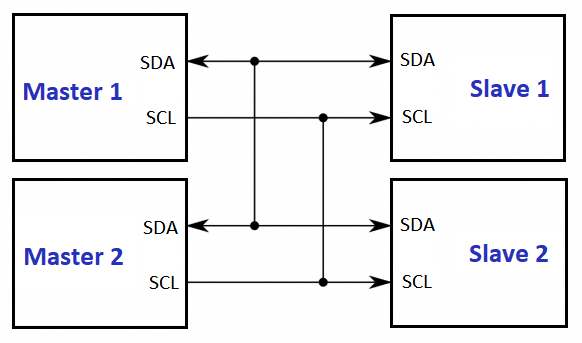
\includegraphics[width=\textwidth]{I2C-Dual-Master}
	\caption{I2C Dual Master Setup}
	\label{fig:I2CDMast}
\end{figure}

In Figure \ref{fig:I2CDMast} is I2C setup with two masters. This is a valid setup for two I2C even though the two Masters could start transmitting simultaneously. This works as both master are continuously monitoring their SDA lines, when one master pulls the SDA low while the other expects it to be high they stop transmitting to wait for their turn.\\

By taking the same concept that I2C uses in their data transmission with two masters, it can be modified to make inter device communication seamless.

\subsection{The Implementation}
While looking for options to solve the multiple device transmission problem, I2C seemed to solve all the problems with some small tweaks.\\

To do distance measurements the following steps will be taken.

\begin{itemize}
\item Initialise Decider
\item Identify Nearby
\item Distance Measurements
\item Information Distribution
\end{itemize}

\subsubsection{Initialise Decider}
This step is done to decide which devices is the first to start transmitting. This step can also have I2C multi-master identification builtin but will not be as reliable.\\

A simple solution is to have the lowest or highest ID device in a region start the identify nearby process. Regions will be described in the information distribution.

\subsubsection{Identify Nearby}
The first device transmits a universal identification command (UIDC). This command when received, all devices that heard the transmission start 'slowly' outputting an identification transmission, containing their ID. The original device repeats everything it hears to make sure all devices that received the original command can hear each other.\\

If any of the devices detect a high output when they have gone low, they will stop transmitting. Since each device has a unique ID, eventually all but one of the devices will stop transmitting. Once the original device identifies another device, it will send out another transmission disabling the device from responding to the next UIDC. Then the whole process repeats until the original device no longer gets a response.

\begin{figure}[h!]
	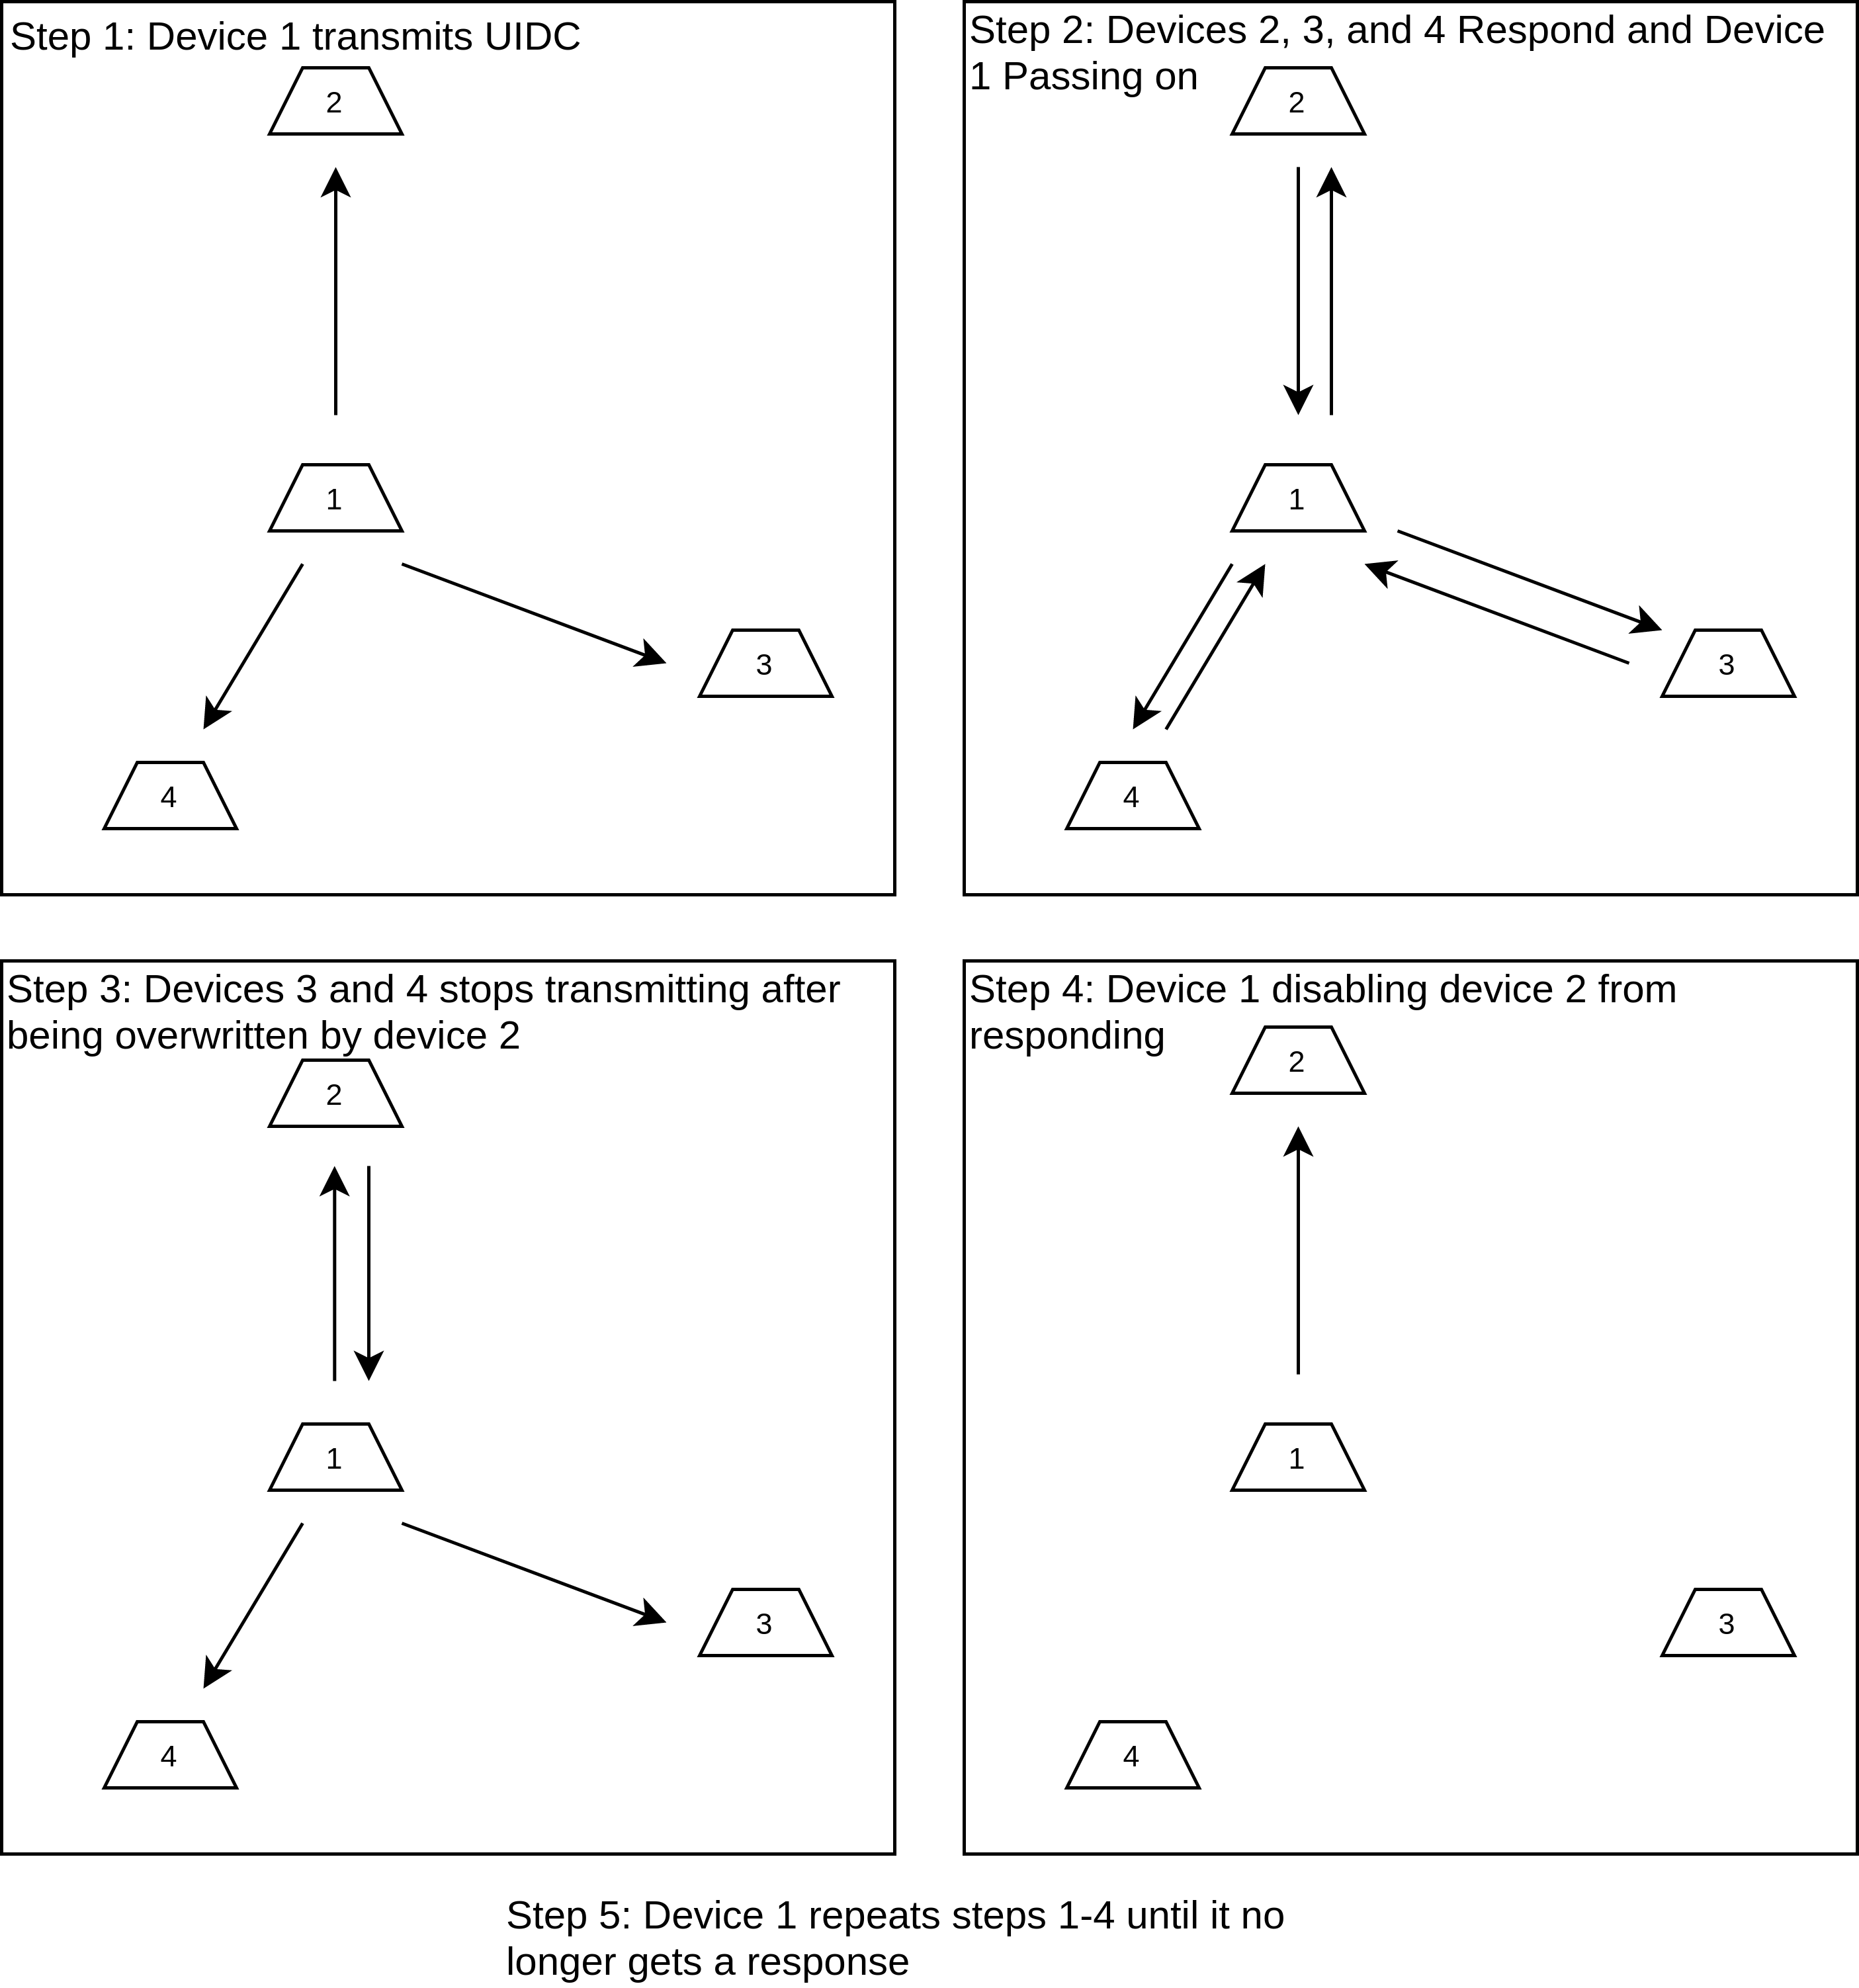
\includegraphics[width=\textwidth]{ID-Process}
	\caption{Multi-device identification process example}
	\label{fig:IDProcess}
\end{figure}

\subsubsection{Distance Measurements}
With all the devices identified, the next step if for the original device to iterate through all IDed devices and measure the distances between each of the devices.\\


\begin{figure}[!h]
	\centering
	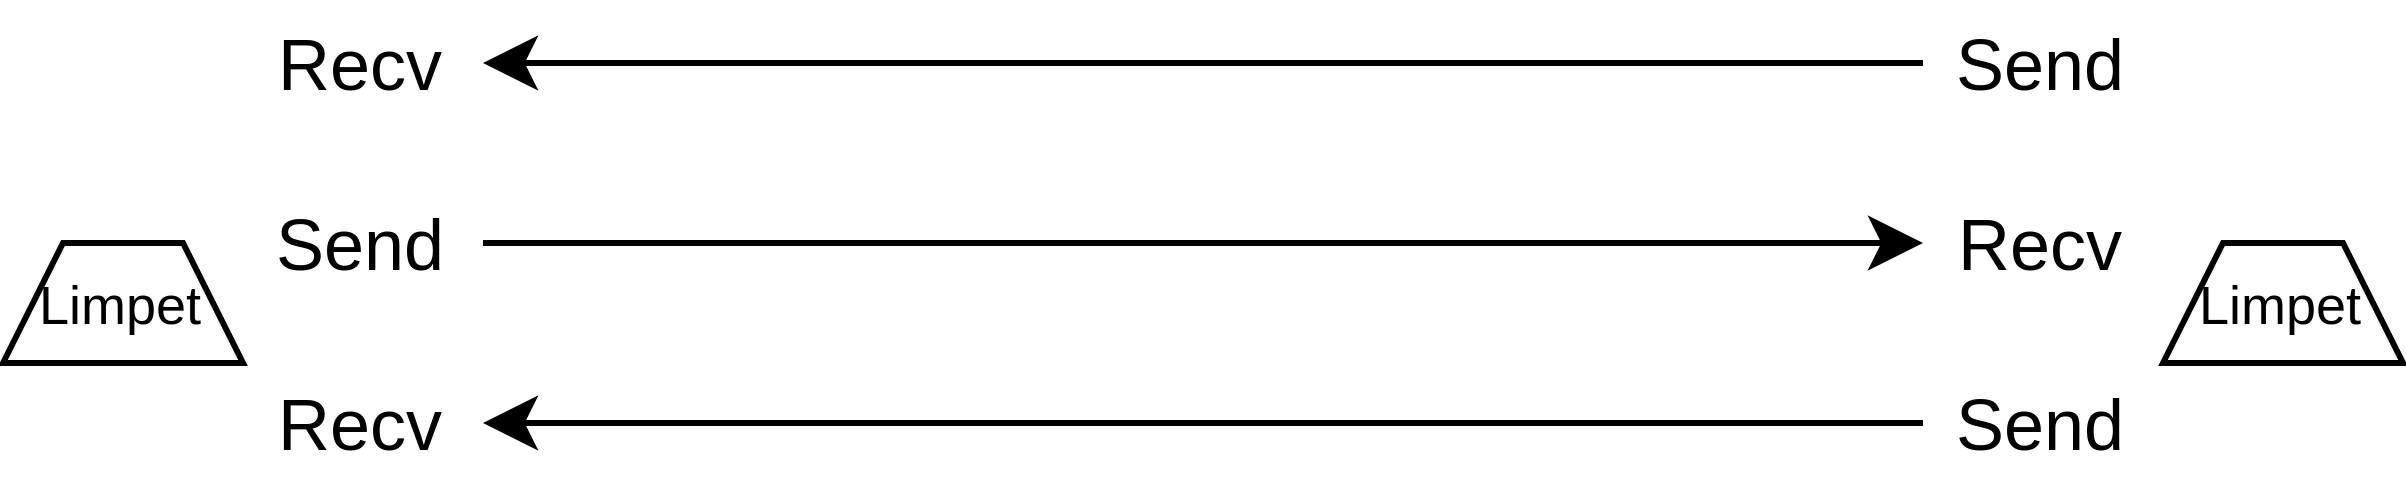
\includegraphics[width=200px]{TriLimpet}
	\caption{Triple back and forth between limpets}
	\label{fig:TriLimp}
\end{figure}

To do the distance measurement, the process previously discussed shown in Figure \ref{fig:TriLimp}. The triple back and fourth gives both limpets the distance.

\subsubsection{Information Distribution}
The final step is important to allow the network to not require all devices to be connected to the network to upload their distances measurements. The following process is done by the device:

\begin{enumerate}
	\item Transmit all measurements and associated IDs to all devices in range
	\item Transmit a command to the next lowest or highest IDed device to identify nearby and do distance measurements.
	\item Sleep until another information distribution occurs.
\end{enumerate}

This list is only partially completed as it requires further development and has started expanding outside of just how the devices communicate and more into how the network interacts.

\subsection{Further Development}
The current approach to implementation doesn't account for properly deciding which device should start next after any given device has finished collecting distance measurements. This require more research/development/design to completed.

\end{document}